\documentclass[11pt]{article}
\usepackage{enumerate}
\usepackage{fullpage}
\usepackage{fancyhdr}
\usepackage{amsmath, amsfonts, amsthm, amssymb}
\usepackage{color}
\usepackage[]{graphicx}

\setlength{\parindent}{0pt}
\setlength{\parskip}{5pt plus 1pt}
\pagestyle{empty}

\def\indented#1{\list{}{}\item[]}
\let\indented=\endlist

\newcounter{questionCounter}
\newcounter{partCounter}[questionCounter]
\newenvironment{question}[2][\arabic{questionCounter}]{%
    \setcounter{partCounter}{0}%
    \vspace{.25in} \hrule \vspace{0.5em}%
        \noindent{\bf #2}%
    \vspace{0.8em} \hrule \vspace{.10in}%
    \addtocounter{questionCounter}{1}%
}{}
\renewenvironment{part}[1][\alph{partCounter}]{%
    \addtocounter{partCounter}{1}%
    \vspace{.10in}%
    \begin{indented}%
       {\bf (#1)} %
}{\end{indented}}

%%%%%%%%%%%%%%%%%%%%%%%HEADER%%%%%%%%%%%%%%%%%%%%%%%%%%%%%%
\newcommand{\myname}{Shashank Singh}
\newcommand{\myandrew}{sss1@andrew.cmu.edu}
\newcommand{\myclass}{86-595 Neural Data Analysis}
\newcommand{\myhwnum}{4}
\newcommand{\duedate}{Thursday, October 18, 2012}
%%%%%%%%%%%%%%%%%%%%%%%%%%%%%%%%%%%%%%%%%%%%%%%%%%%%%%%%%%%

%%%%%%%%%%%%%%%%%%%%CONTENT MACROS%%%%%%%%%%%%%%%%%%%%%%%%%
\newcommand{\ans}[1]{\mbox{\fbox{$\displaystyle #1$}}} % box around an answer in math mode
\renewcommand{\qed}{\quad $\blacksquare$} % black QED square
\newcommand{\mqed}{\quad \blacksquare} % black QED square for use in math mode
\newcommand{\inv}{^{-1}} % inverse
\newcommand{\blambda}{\boldsymbol{\lambda}}
\newcommand{\br}{\mathbf{r}}
\newcommand{\bx}{\mathbf{x}}
\newcommand{\by}{\mathbf{y}}
\newcommand{\bff}{\mathbf{f}}
\newcommand{\bzero}{\mathbf{0}}
\newcommand{\N}{\mathbb{N}} % natural numbers
\newcommand{\Q}{\mathbb{Q}} % rational numbers
\newcommand{\R}{\mathbb{R}} % real numbers
\newcommand{\E}[1]{\mathsf{E}\left[#1\right]} % expected value
\newcommand{\Var}[1]{\mathsf{Var}\left[#1\right]} % variance
\newcommand{\Poisson}[1]{\operatorname{Poisson}\left(#1\right)} % Poisson distribution
\newcommand{\Exp}[1]{\operatorname{Exp}\left(#1\right)} % Exponential distribution
\newcommand{\U}[2]{\operatorname{U}\left(#1,#2\right)} % Uniform distribution
\newcommand{\Bern}[1]{\operatorname{Bernoulli}\left( #1 \right)} % Bernoulli distribution
\newcommand{\pr}[1]{\mathsf{P}\left( #1 \right)} % probability of event #1
\newcommand{\argmax}{\operatornamewithlimits{argmax}}
\newcommand{\argmin}{\operatornamewithlimits{argmin}}
%%%%%%%%%%%%%%%%%%%%%%%%%%%%%%%%%%%%%%%%%%%%%%%%%%%%%%%%%%%

\begin{document}
\thispagestyle{plain}

{\Large Homework \myhwnum} \\
\myclass \\
Name: \myname \\
Email: \myandrew \\
Due: \duedate \\
\begin{question}{Problem 1}
\begin{enumerate}[a.]
\item Since each neuron is independent, by properties of logarithms,
\begin{align*}
\ell(s)
 & = \ln \left( \pr{\br | \blambda(s)} \right)
   = \ln \left( \prod_i \pr{r_i | \lambda_i(s)} \right)
   = \sum_i \ln \left( \pr{r_i | \lambda_i(s)} \right) \\
 & = \sum_i \ln \left( \frac{\lambda_i^{r_i}(s)}{r_i!}e^{-\lambda_i(s)} \right)
   = \sum_i r_i \ln \left( \lambda_i(s) \right) - \lambda_i(s) - \ln(r_i!).
     \mqed
\end{align*}

\item By the result of part a., since $\sum_i \lambda_i(s)$ and
$\sum_i \ln(r_i!)$ are constant with respect to $s$,
\[\hat{s}_{ML}
 = \argmax_s \ell(s)
 = \argmax_s \sum_i r_i \ln \left( \lambda_i(s) \right).
\]
Then, by definition of $\lambda_i(s)$, since $2\sigma^2$ is constant with
respect to $s$,
\[\hat{s}_{ML}
 = \argmax_s \sum_i r_i \ln \left( \exp \left( \frac{(s - \mu_i)^2}{2\sigma^2} \right) \right)
 = \argmax_s \sum_i r_i \frac{(s - \mu_i)^2}{2}.
\]
Assuming this function achieves its maximum at the zero of its derivative
gives
\[0
 = \sum_i r_i (\hat{s}_{ML} - \mu_i)
 = \sum_i r_i \hat{s}_{ML} - \sum_i r_i \mu_i,
    \quad \mbox{so that} \quad
\hat{s}_{ML} = \frac{\sum_i r_i \mu_i}{\sum_i r_i}. \mqed\]

\item As shown in part b.,
\begin{align*}
\hat{s}_{MAP}
 & = \argmax_s \ell(s) p(s)
   = \argmax_s \ln (\ell(s) p(s))
   = \argmax_s \ln \ell(s) + \ln p(s) \\
 & = \argmax_s \sum_i \frac{r_i(s - \mu_i)^2}{2\sigma^2} + \ln \left( \exp \left( \frac{(s - s_{prior})^2}{2\sigma_{prior}^2} \right) \right) \\
 & = \argmax_s \sum_i \frac{r_i(s - \mu_i)^2}{2\sigma^2} + \frac{(s - s_{prior})^2}{2\sigma_{prior}^2}.
\end{align*}
Assuming this function achieves its maximum at the zero of its derivative
gives
\[0
 = \sum_i \frac{r_i(\hat{s}_{MAP} - \mu_i)}{\sigma^2} + \frac{(\hat{s}_{MAP} - s_{prior})}{\sigma_{prior}^2},
    \quad \mbox{so that} \quad
\hat{s}_{MAP} = \frac{\sum_i\frac{r_i\mu_i}{\sigma^2} + \frac{s_{prior}}{\sigma_{prior}^2}}{\sum_i \frac{r_i}{\sigma^2} + \frac{1}{\sigma_{prior}}}. \mqed
\]

\end{enumerate}
\end{question}

\begin{question}{Problem 2}
\begin{enumerate}[a.]
\item The following matlab code computes, for each firing rate, the difference
between the likelihoods $\pr{f | A} - \pr{f | B}$. If this is difference is
positive, $\ell(A) > \ell(B)$, so MLE predicts the stimulus as A;
otherwise, MLE predicts the stimulus as B.
\begin{verbatim}
>> f = [2 5 8 11 14 17];
>> ma = 8; sa = 5; mb = 12; sb = 6;
>> L = (1/sa)*exp(-(f - ma).^2/(2*sa^2)) - (1/sb)*exp(-(f - mb).^2/(2*sb^2));
>> [f; L > 0]

ans =
     2     5     8    11    14    17
     1     1     1     1     0     0
\end{verbatim}
Thus we have
\begin{center}
\begin{tabular}{|c|c|c|c|c|c|c|}
\hline
$f [sp/s]$ & 2 & 5 & 8 & 11 & 14 & 17 \\
\hline
 MLE       & A & A & A &  A &  B &  B \\
\hline
\end{tabular}.
\end{center}

\item If, instead, we compute the posteriors by myltiplying the likelihoods by
the priors, the matlab code gives:
\begin{verbatim}
>> P = (1/3)*(1/sa)*exp(-(f - ma).^2/(2*sa^2))...
                                    - (2/3)*(1/sb)*exp(-(f - mb).^2/(2*sb^2));
>> [f; P > 0]

ans =
     2     5     8    11    14    17
     1     0     0     0     0     0
\end{verbatim}
Thus we have
\begin{center}
\begin{tabular}{|c|c|c|c|c|c|c|}
\hline
$f [sp/s]$ & 2 & 5 & 8 & 11 & 14 & 17 \\
\hline
 MAP       & A & B & B &  B &  B &  B \\
\hline
\end{tabular}.
\end{center}

\end{enumerate}
\end{question}

\begin{question}{Problem 3}
\begin{enumerate}[A)]
\item
\begin{enumerate}[i)]
\item Since Na\"ive Bayes assumes that the $X_i$'s are conditionally
independent given $Y$,
\[\pr{X | Y} = \pr{X_1,X_2,\dots,X_n | Y} = \ans{\prod_i \pr{X_i | Y}.}\]

\item Since we are only interested in computing $\argmax_Y \pr{Y | X}$, and
$\pr{X}$ is constant with respect to $Y$, we can ignore the $\pr{X}$ in the
denominator.

\item By the result of part a.,
\[\pr{X = x_i | Y = y} \pr{Y = y}
 = \ans{\pr{Y = y} \prod_i \frac{\lambda_{i,y}^{x_i}}{x_i!}e^{-\lambda_{i,y}}.}
\]

\item Using the result of part a. of Problem 1 gives
\begin{align*}
\ln (\pr{X | Y} \pr{Y})
 & = \ln \pr{Y = y} + \ln \left( \prod_i \frac{\lambda_{i,y}^{x_i}}{x_i!}e^{-\lambda_{i,y}} \right) \\
 & = \ans{\ln \pr{Y = y} + \sum_i x_i \ln \left( \lambda_{i,y} \right) - \lambda_{i,y} - \ln(x_i!).}
\end{align*}
\end{enumerate}

%TODO
\item
\begin{enumerate}[i)]
\item The following is my implementation of \texttt{trainPoissonNBDecoder}:
{\footnotesize
\begin{verbatim}
function [classMeans, classPriors] = trainPoissonNBDecoder(trainCounts, trainLabels)

  classes = unique(trainLabels); % this way generalizes to multiple classes

  for i=1:length(classes)
    classMeans(:,i) = mean(trainCounts(:,trainLabels ==  classes(i)),2);
    classPriors(i) = sum(trainLabels == i)./length(trainLabels);
  end
end
\end{verbatim}
}

\item The following is my implementation of \texttt{poissonNBDecode}:
{\footnotesize
\begin{verbatim}
function estLabels = poissonNBDecode(testCounts, classMeans, classPriors)

  l = zeros(size(testCounts,2),length(classPriors));

  for trial=1:size(testCounts,2)
    gln = gammaln(testCounts + 1);

    for class=1:length(classPriors)
      l(trial, class) = testCounts(:,trial)'*log(classMeans(:,class)); % xln(lambda)
      l(trial, class) = l(trial,class) - sum(classMeans(:,class)); % - lambda
      l(trial, class) = l(trial,class) - sum(gln(:,trial)); % - ln(x!)
    end
    posterior(trial,:) = log(classPriors) + l(trial,:);
  end

  [~, estLabels] = max(posterior',[],1);
end
\end{verbatim}
}

\item The decoder is \ans{80.2\%} accurate.

\item
See Figure~\ref{fig:3Biv}.
\begin{figure}[h]
\begin{center}
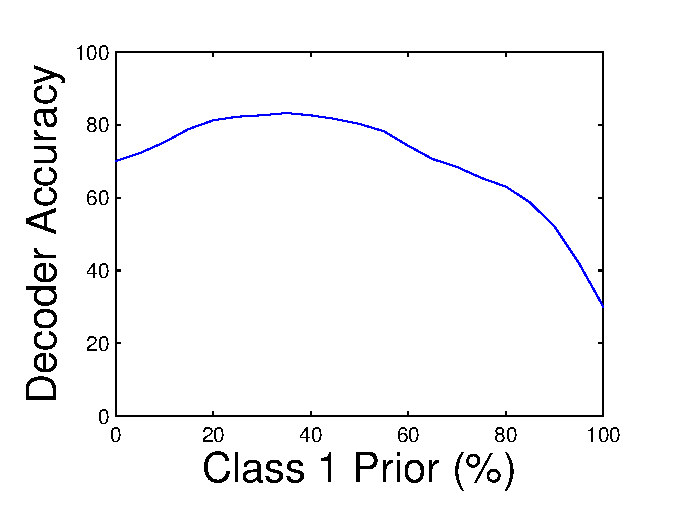
\includegraphics[width=0.46\textwidth]{3Biv}
\end{center}
\caption{Decoding accuracy for different class 1 priors.}
\label{fig:3Biv}
\end{figure}

\item Decoding accuracy is maximized when the class 1 prior is $35\%$ (so that
the class 2 prior is $65\%$), which is significantly lower than the prior
learned from the training data ($50\%$ each for class 1 and class 2). This
makes sense since looking at \texttt{testLabels} reveals that only 150 of the
500 test examples ($30\%$) were from class 1, whereas about 250 of the 500
training examples ($50\%$) were from class 1. In this case, the difference in
test accuracies using our learned prior and the optimal prior was only $3\%$,
so it was not very signficant, but, had the learned class 1 prior been much
greater, the difference could have been as much $50\%$, so knowing the true
prior may be more important in general.

\item Since spike data is inevitably noisy, there will always be class 1
trials with spike counts resembling class 2 trials, and vice versa.
Furthermore, Na\"ive Bayes can only fit a linear decision surface, which
may not be sufficiently descriptive to classify the data. Approaches to
increasing decode accuracy might include reducing noise in both the training
and test data (e.g., spike sorting) or using a more powerful classifer (e.g.,
a nonlinear classifier, or one that does not make Na\"ive Bayes conditional
independence assumptions; relaxing the conditional independence assumptions
may be particularly important, since neurons are known to have significant
noise correlation).
\end{enumerate}
\end{enumerate}
\end{question}

\begin{question}{Problem 4}
This homework was pretty short; the theory questions went very quickly, and
the only part of the coding that took me a while was remembering that
$\Gamma(n) = (n - 1)!$, not $n!$, which brought my decoding accuracy down to
$64\%$ in part iii).

I'm also taking a Machine Learning class (10-601) alongside, so I've seen and
implemented MLE, MAP, and Na\"ive Bayes before, although I haven't done so
with neural data, so deriving the solutions for the Poisson case was nice.
But how reasonable is the assumption that the neurons' tuning curves uniformly
tile the stimulus space? I do research in visual cortex, where this is almost
never the case.

I was a little confused because part iv) of the coding section seemed to have
already been implemented in the script; were we supposed to do anything more
for that part than attach the plot generated?
\end{question}
\end{document}
